\section{Experiments}

% Main results table. Generated from the run sheet; totals verified against
% the per-task numbers. Requires \usepackage{booktabs}.
%
% Uniform = static 1/K mixture; Single = per-task specialists (confirmed).
\begin{table}[t]
\centering
\caption{\textbf{Multi-task post-training results.} Per-task accuracy (\%) on the
Nemo-Gym (four tasks) and ACZ (three tasks) suites, at pass@1 and pass@4.
\textbf{PDCM} is our method; \textbf{Uniform} holds the mixture fixed at $u=1/K$,
\textbf{Single} trains one specialist per task, \textbf{PCGrad}~\citep{pcgrad2020}
resolves gradient conflicts, and \textbf{Aioli}~\citep{chen2025aioli} allocates under a
parametric mixing law. Per row, the best result is in \textbf{bold} and the second best is
\underline{underlined}; \emph{Total} is the sum over a suite's tasks.}
\vspace{0.2cm}
\label{tab:main}
\footnotesize
\setlength{\tabcolsep}{3pt}
\begin{tabular}{l rrrrr rrrrr}
\toprule
 & \multicolumn{5}{c}{pass@1} & \multicolumn{5}{c}{pass@4} \\
\cmidrule(lr){2-6} \cmidrule(lr){7-11}
Task & PDCM & Uniform & Single & PCGrad & Aioli & PDCM & Uniform & Single & PCGrad & Aioli \\
\midrule
\multicolumn{11}{l}{\textit{Nemo-Gym}} \\
\texttt{code\_gen} & 32.61 & 34.08 & 31.29 & \underline{34.39} & \textbf{35.40} & \textbf{43.50} & 41.41 & 37.73 & 42.43 & \underline{43.29} \\
\texttt{IF} & \textbf{53.33} & 47.58 & 36.63 & \underline{51.00} & 47.79 & \textbf{60.38} & 54.57 & 45.76 & \underline{58.81} & 52.09 \\
\texttt{workplace} & \textbf{82.89} & 81.74 & \underline{82.61} & 74.72 & 82.11 & 83.35 & 84.00 & \underline{86.46} & 75.15 & \textbf{87.97} \\
\texttt{xlam} & \textbf{84.35} & 74.87 & \underline{83.57} & 82.92 & 82.32 & \textbf{84.28} & 80.70 & 83.91 & 83.19 & \underline{84.10} \\
\cmidrule(lr){1-11}
Total & \textbf{253.18} & 238.27 & 234.10 & 243.03 & \underline{247.62} & \textbf{271.51} & 260.68 & 253.86 & 259.58 & \underline{267.45} \\
\midrule
\multicolumn{11}{l}{\textit{ACZ}} \\
ARC-1D & \textbf{66.33} & \underline{61.28} & 50.08 & 29.29 & 58.17 & \textbf{80.37} & \underline{77.39} & 66.60 & 39.88 & 70.53 \\
Countdown & \underline{91.83} & 91.06 & 88.09 & 89.92 & \textbf{92.33} & \underline{94.48} & 94.43 & 91.80 & 92.69 & \textbf{94.56} \\
Zebra & \underline{91.08} & \textbf{91.12} & 87.79 & 79.42 & 90.54 & \textbf{97.21} & 96.68 & 95.47 & 89.25 & \underline{96.91} \\
\cmidrule(lr){1-11}
Total & \textbf{249.24} & \underline{243.46} & 225.96 & 198.63 & 241.04 & \textbf{272.06} & \underline{268.50} & 253.87 & 221.82 & 262.00 \\
\bottomrule
\end{tabular}
\end{table}



\subsection{Datasets}
\label{sec:datasets}

\paragraph{Nemo-Gym.}~\citep{nemogym}
We selected four heterogeneous tasks served from the NeMo-Gym servers, some requiring tool-use or multi-turn capabilities, some do not.
\textbf{\texttt{IF}} draws its training prompts from the WildChat-1M dataset~\citep{zhao2024wildchat1mchatgptinteraction} with instructions from the Open-Instruct code base~\citep{ahmad2025opencodeinstructlargescaleinstructiontuning}, and is evaluated on the held-out IF-Bench~\citep{ifbench}. \textbf{\texttt{code\_gen}} contains competitive coding challenges from
NVIDIA's OpenCodeReasoning~\citep{ahmad2025opencodereasoningadvancingdatadistillation} dataset. This dataset is served with Nemo-Gym's single-turn verification engine \texttt{code\_gen}.
\textbf{\texttt{xlam\_fc}}~\citep{zhang2024xlamfamilylargeaction} is an API/function calling dataset in xLAM format.
\textbf{\texttt{workplace}}~\citep{nemogym} is a tool-use multi-step agentic environment that tests the agent’s ability to execute tasks in a workplace setting such as calendar scheduling or email management.
Tab.~\ref{tab:agentic} (App.~\ref{app:agentic-data}) lists the per-task train and test sizes.


\paragraph{Reasoning-Gym.}~\citep{reasoninggym}
Our reasoning mixture is procedurally generated with scripts offered by Reasoning-Gym~\citep{reasoninggym}.
Each task is instantiated at three difficulty levels (easy, medium, and hard) with 30000 training and 600 test problems. We describe the individual tasks below.
\textbf{\textit{ARC-1D}} is an abstract pattern-induction puzzle where the agent infers the grid transformation rule from examples.
\textbf{\textit{countdown}} is a numbers game in which the agent combines given numbers and fixed set of operations to hit a target.
\textbf{\textit{zebra}} a logic game where you use clues and deduction to match attributes across different colored houses.
\textbf{\textit{word\_sorting}} is an alphabetical word-sorting task.
In \textbf{\textit{puzzle24}}, one needs to combine four numbers and basic arithmetic operations to make 24. 
In \textbf{\textit{manipulate\_matrix}}, one must apply given grid operations in sequence to reach a given state.
App.~\ref{app:rg-generation} reports the complete generation configurations.

\subsection{Experimental Setup}
\begin{wrapfigure}{r}{0.42\textwidth}
  \vspace{-\intextsep}
  \centering
  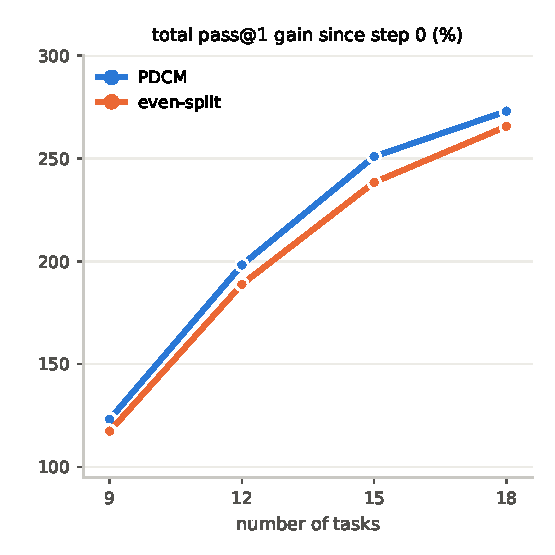
\includegraphics[width=0.40\textwidth]{fig/pdcm_scaling.pdf}
  \caption{\textbf{Scaling with mixture size.} PDCM stays above the even-split
  ($1/K$) baseline at every $K$.}
  \label{fig:scaling}
  \vspace{-1cm}
\end{wrapfigure}
All Experiments are run using Qwen3-4B with thinking turned off. The main experiments are run on two H200 with a training budget of 48 hours, unless otherwise noted.
For the Nemo-Gym mixture, PDCM and Aioli control the allocation quota of each dataset. On
Reasoning-Gym, we find that averaging $\widehat U_{t,k}$ over difficulty levels erase
the vital policy signal PDCM relies on for allocation. We
therefore let the allocation methods control each difficulty level directly, so a $K$-task
Reasoning-Gym mixture is effectively a $3K$-unit allocation problem.
\vspace{-0.3cm}


\subsection{Baselines}

All methods share the model, RL algorithm, data pools, and training budget, and differ only in
how the per-step mixture is chosen or how the resulting updates are combined.

\textbf{Uniform} is a multi-task baseline that fixes the mixture at $u=1/K$ for the whole run.

\textbf{Single} trains one specialist per task: $K$ separate runs, each with $1/K$ of
multi-task methods' data budget.

\textbf{PCGrad}~\citep{pcgrad2020} holds the mixture uniform and intervenes on the update
instead, projecting conflicting task gradients onto one another's normal plane. It represents
the gradient-surgery family.

\textbf{Aioli}~\citep{chen2025aioli} is the closest prior allocation method. Like PDCM it
adjusts the mixture online, but it does so through the parametric mixing law.

\begin{figure}[t]
  \centering
  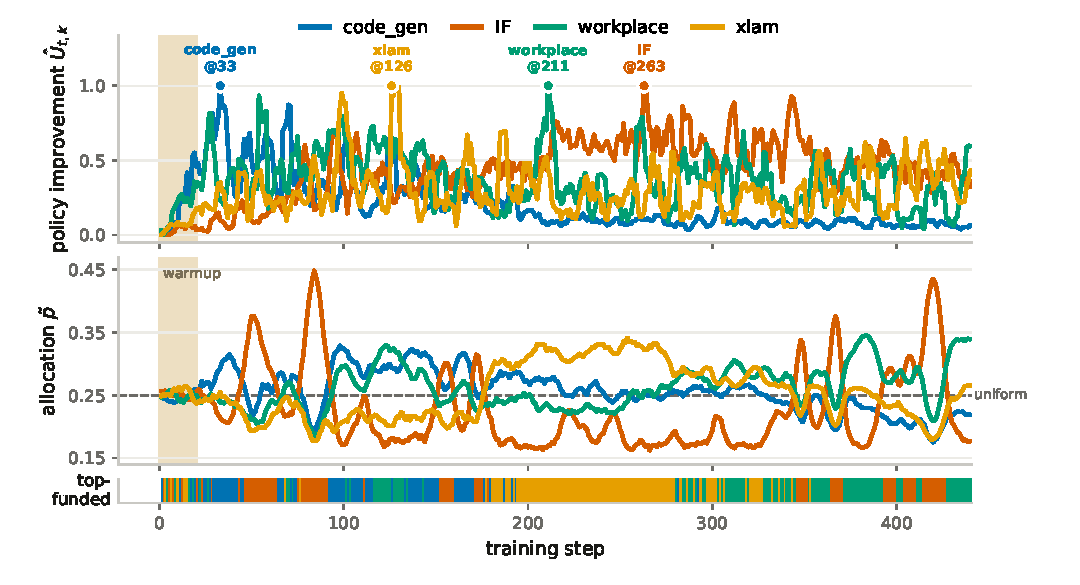
\includegraphics[width=\linewidth]{fig/pdcm_dynamics.pdf} % <- adjust path
  \caption{\textbf{PDCM rides a non-stationary improvement landscape.}
  A four-task mixture (Qwen3-4B, GSPO, $440$ steps).
  \textbf{(a)} Per-task one-step improvement $\hat U_{t,k}$ (normalized within task;
  the raw signals differ by ${\sim}20\times$ in scale), with each task's peak window
  marked. The high-improvement window rotates across tasks over training.
  \textbf{(b)} PDCM's applied allocation $\tilde p_t$, bounded by the floor/cap
  ($[0.15,0.55]$) and oscillating about the uniform $1/K$; the time-average is
  near-uniform despite continual reallocation.
  \textbf{(c)} The top-funded task over time. Leadership rotates
  (${\sim}100$ switches) with coarse structure that tracks (a) for
  $\texttt{xlam}$ (mid), $\texttt{workplace}$ (late), and $\texttt{code\_gen}$
  (defunded as it saturates); $\texttt{instruction\_following}$ is the exception
  (Sec.~\ref{sec:dynamics}).}
  \label{fig:dynamics}
\end{figure}

\subsection{Allocation Dynamics}
\label{sec:dynamics}

We study the allocation dynamics of PDCM on the 4-task Nemo-Gym mixture. As shown in Fig.~\ref{fig:dynamics}, the allocation can be roughly broken down into three phases.
\begin{enumerate}
    \item Through the first $200$ steps $\texttt{code\_gen}$ is most often top-funded, induced by its large improvements early in training.
    \item Between steps $200$ and $300$ leadership passes to $\texttt{xlam}$, whose measured improvement degrades when it is under-allocated, which sustained its continual allocation. 
    \item Once $\texttt{xlam}$'s policy improvement was able to grow without further allocation, $\texttt{workplace}$ becomes the best-funded task for the remainder of the run around step 300.
\end{enumerate}

Three of the four tasks thus receive a dominant phase. The
exception, $\texttt{IF}$'s proportion oscillates between $0.15$ and $0.45$, and these spurts of
budget are enough for it to maintain lead against the mixed baseline. Across all
four, the \emph{time-averaged} allocation remains nearly uniform (every task
within $\pm0.01$ of $1/K$). The near-uniform mean indirectly support that the
no-task-left-behind constraint of \Cref{eq:constraint_uniform_baseline} takes effect.